\mychapter{1}{Introduction}
In the Paris Agreement of 2015, 195 countries and their governments agreed on global efforts to reduce the amount of carbon dioxide (CO$_2$) emitted into the atmosphere, with the goal of limiting global atmospheric warming to "well below" 2 °C, ideally 1.5 °C, compared to the pre-industrial baseline.\vspace{2mm}

Although the primary imperative of the agreement is emission abatement, including the decarbonization of key industries and the transport sector, many projections increasingly factor in the use of negative emissions technologies (NETs), also known as carbon dioxide removal (CDR), which remove CO$_2$ from the atmosphere \parencite{unep_emissions_2017}. These technologies are projected to be used to counterbalance the about 10\% "hard-to-abate residual" CO$_2$ emissions from industries such as air travel and transport, whose decarbonization is not economically feasible \parencite{prutz_understanding_2023}. This means that between the present day and the mid-century, NETs must be developed from proofs-of-concept and pilot plants to a Gigatons-per-year industry in order to acomplish the goals of the Paris Agreement.

\section{The Spectrum of Carbon Removal}
Carbon removal is still a relatively early-stage industry with a vast and often obscure landscape of actors, who use a wide variety of approaches to generate offsetting claims on carbon dioxide ("carbon credits"), which range from the simple avoidance of deforestation, over investments in renewable energies, to complex, novel technologies such as Direct Air Capture (DAC). For example, many airlines offer passengers to offset the CO$_2$ caused by their flights for an additional cost of only a few dollars \parencite{evz_offsetting_2023}. However, these offsets are typically of questionable value and hard to quantify regarding the real climate impact and permanence \parencite{trencher_demand_2024}.\vspace{2mm}

This thesis focuses on negative emissions technologies (NET's), which deliver quantifiable negative emissions by actually removing CO$_2$ from the atmosphere and storing it for a sufficiently long time frame to be considered permanent. The term negative emissions technologies itself encompasses a wide range of diverse approaches, which can generally be classified on a spectrum going from enhanced natural sinks to engineered (so-called "novel") carbon removal technologies. This thesis focuses on four distinct approaches that are sufficiently advanced on the maturity curve, represent the structural trade-offs of the sector, and have seen the most research and adoption so far: Afforestation and Reforestation (A/R), Enhanced Rock Weathering (ERW), Biomass Carbon Removal and Storage (BiCRS), and Direct Air Capture (DAC).\vspace{2mm}

A/R involves the restoration of previously deforested areas, either through natural regeneration or manual plantation, and represents the fully natural side of the spectrum. Carbon removal is achieved through biomass accumulation, which is considered a mature and well-understood process. Trade-offs include the constant reversal risk due to wildfires or droughts, which threaten the permanence of the stored carbon, as well as the question of land-use competition and biodiversity in case of large-scale deployment \parencite{gunther_carbon_2024}.\vspace{2mm}

In contrast, DAC is situated on the entirely engineered end of the spectrum. It uses chemical sorbents or solvents (in solid and liquid DAC, respectively) to strip CO$_2$ directly from the ambient air. It is thermodynamically challenging due to the low concentration of CO$_2$ in the atmosphere \parencite{lackner_thermodynamics_2013}, but offers a high verifiability and durability, as well as location flexibility. However, it is currently prohibitively expensive and still requires significant capital investments and development efforts to achieve a learning-curve-based cost reduction and energy cost optimization \parencite{lackner_buying_2021, babacan_role_2020}\vspace{2mm}

Finally, ERW and BiCRS occupy a hybrid space. ERW uses ground silicate rock materials, spread out on large land areas, to accelerate the natural geological weathering process, converting atmospheric CO$_2$ to stable, dissolved carbonates \parencite{larkin_carbon_2023}. This method is both deployable at scale and verifiably permanent, but entails significant logistical challenges comparable to the global mining industry \parencite{madankan_larger_2025}. BiCRS entails approaches such as Bioenergy with Carbon Capture and Storage (BECCS) and Biochar, and uses biomass to store carbon through either combustion combined with with carbon capture and storage (CCS) or pyrolysis. However, the use of purpose-grown energy crops again poses the risk of land-use competition and biodiversity reduction \parencite{gaucher_leveraging_2025}. For the purpose of this thesis, only BiCRS using waste biomass will be considered.
\begin{table}[]
\small
\renewcommand{\arraystretch}{1.4}
\begin{tabular}{lllll}
Technology     & Classification     & Storage Mechanism   & Storage Durability     & Key Resource Constraint  \\ \hline
\textbf{A/R}   & Nature-Based       & Biomass & Decades   to Centuries & Land, Water             \\
\textbf{ERW}   & Hybrid/Geochemical & Chemical   & Millennia              & Mining Logistics, Energy \\
\textbf{BiCRS} & Hybrid/Industrial  & Geological                  & Centuries to Millennia              & Biomass Supply (Land)   \\
\textbf{DAC}   & Engineered/Novel   & Geological                  & Millennia              & Energy, Capital      \\ \hline  
\end{tabular}
\caption{Classification and characteristics of selected NETs}
\end{table}

\section{Voluntary Carbon Markets and the CDR Governance Paradox}
Voluntary carbon markets (VCM's) are markets in which carbon credits are traded on a voluntary basis. These markets consist of a four types of actors: Project developers, which develop offsetting projects and issue carbon credits; Standard setters, which verify that the credits follow their requirements and often also act as registries, tracking the credits from issuance to retirement; Brokers, which allow credits to be exchanged; and buyers, who retire the credits to offset their carbon emissions.\vspace{2mm}

\begin{figure}[ht]
  \centering
  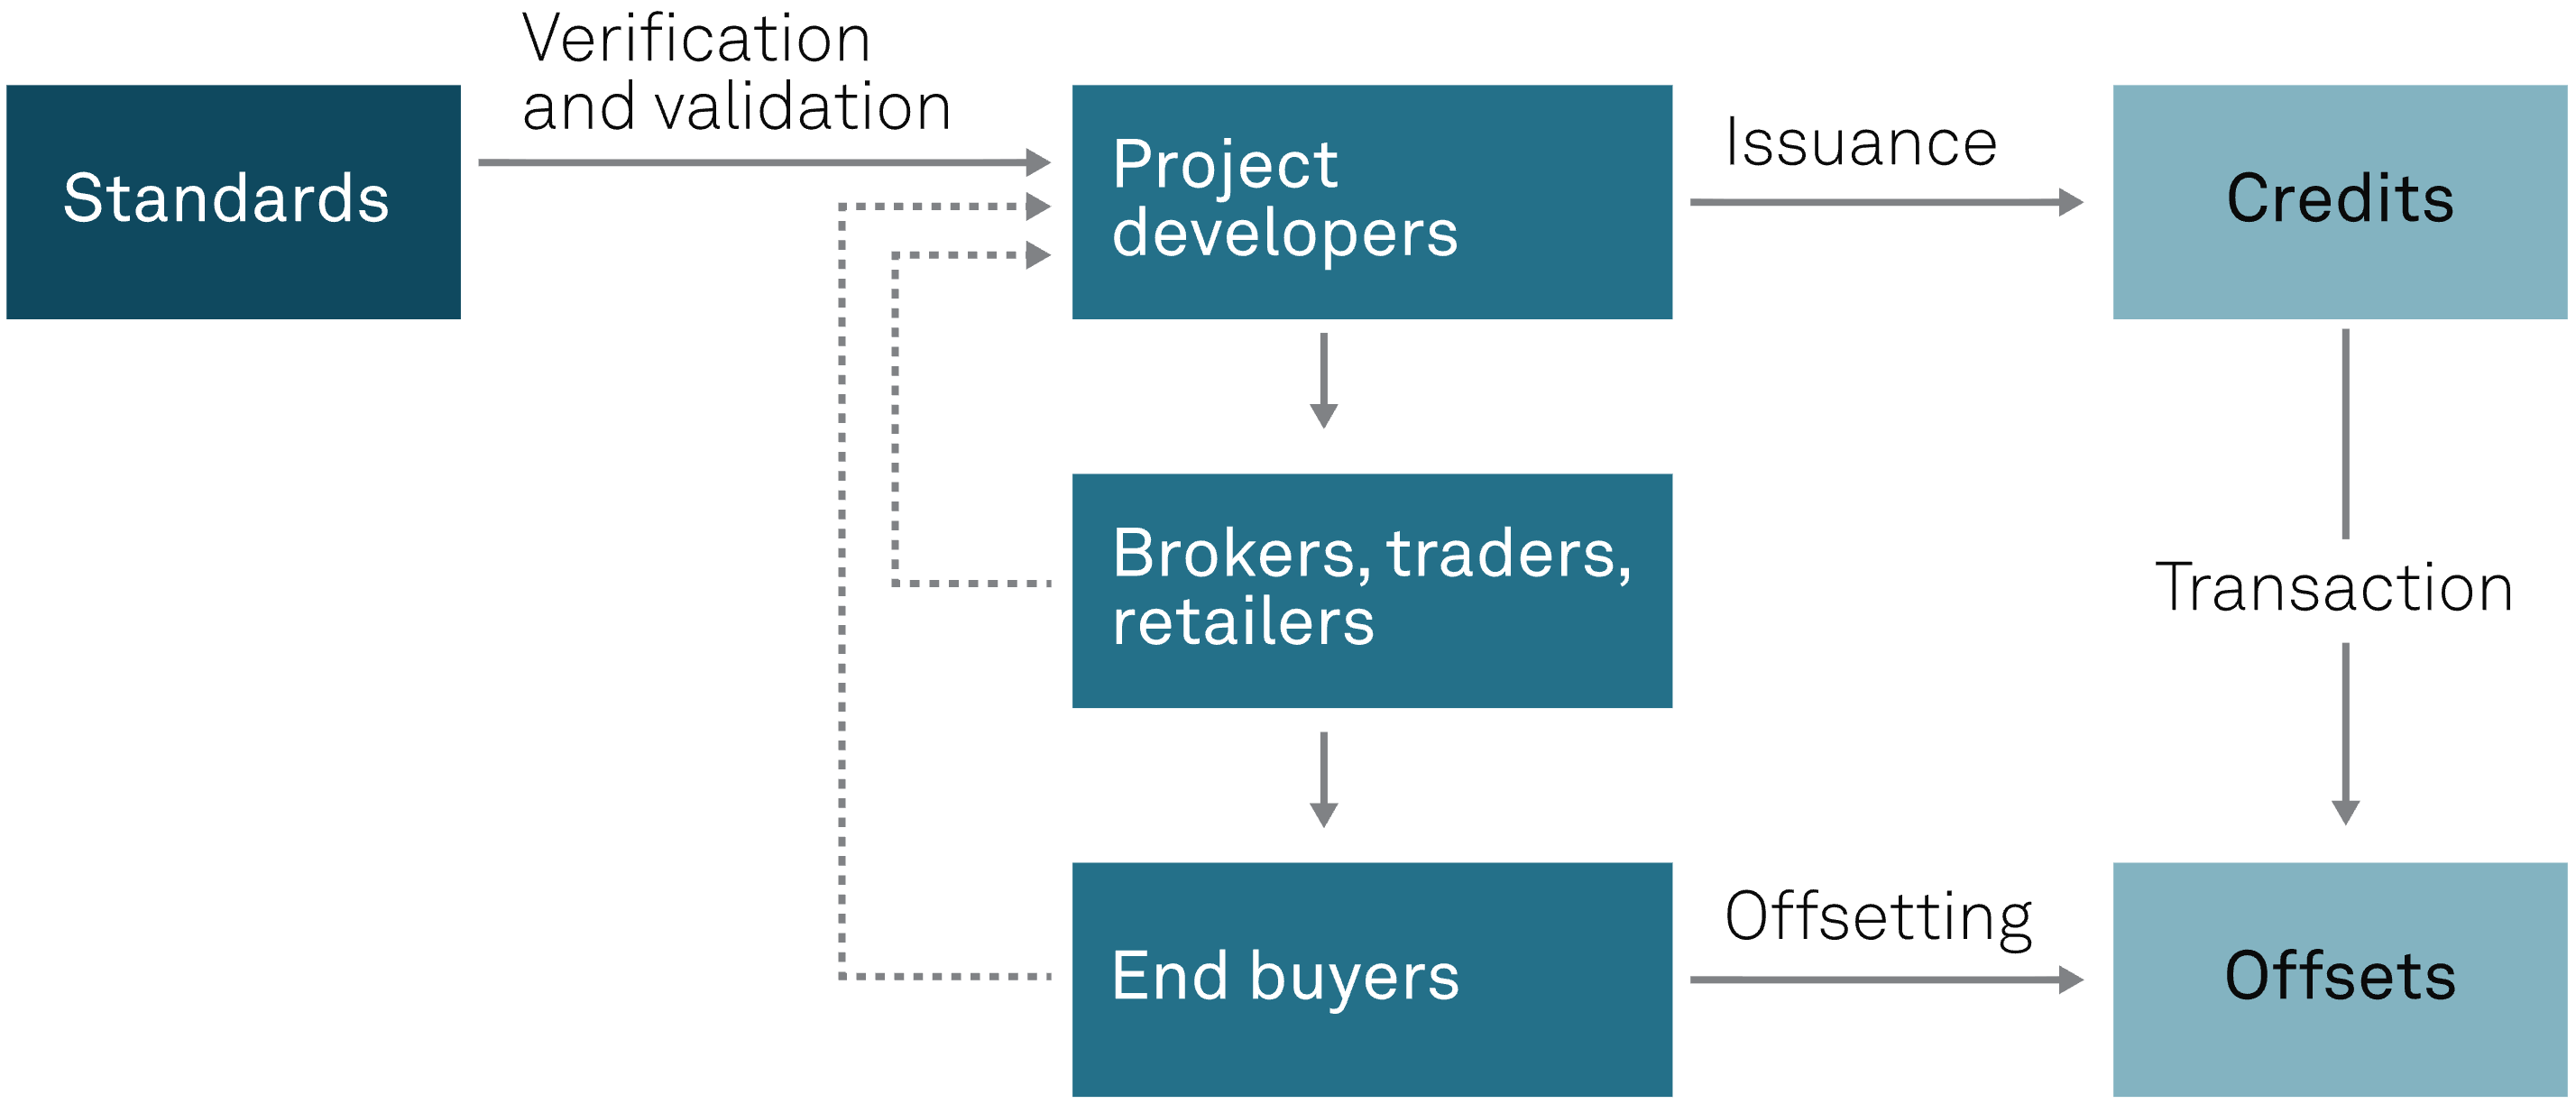
\includegraphics[width=0.7\linewidth]{figures/vcm.png}
  \caption[Structure of voluntary carbon markets]{Structure of voluntary carbon markets, \textit{reproduced from \textcite{favasuli_voluntary_2025} / S\&P Global Energy}}
  \label{fig:usa_sample_case}
\end{figure}

To reliably meet global net-zero goals, CDR governance frameworks must incentivize the investment in and use of NETs that deliver verifiable, permanent removals with a proven additionality, that is, a net-negative effect on atmospheric CO$_2$ levels. The \textit{Oxford principles for net zero aligned carbon offsetting} \parencite{axelsson_revised_2024} specifically call for a one-thousand-fold increase of the amount of high-quality, durable carbon removal and storage until 2050 and clear, internationally-agreed definitions of risks, benefits and terminology of the various CDR approaches.\vspace{2mm}

In contrast, VCM's have historically prioritized volume and price over verifiability and permanence \parencite{chawla_role_2023}. Prices for avoidance credits, which typically involve the buying party paying the selling party for merely avoiding carbon emissions, start at 4 US\$ per tonne\footnote{The spelling "tonne" is used to refer to metrics tons, as opposed to imperial tons.} of CO$_2$, while high-quality credits, which use technologies such as DAC, cost up to 500 US\$ per tonne of CO$_2$ \parencite{reichelstein_accounting_2024}.\vspace{2mm}

This market failure creates four primary problems. First, an expansive supply of avoidance credits, often from questionable forestry projects \parencite{chawla_role_2023}, allows actors to make inflated claims of carbon neutrality while making little to no real impact \parencite{trencher_demand_2024, toussaint_its_2025}. Second, it causes significant accounting issues and uncertainty for investors when comparing carbon neutrality claims of different companies. Compared to established financial accounting standards, such as IFRS, no globally accepted accounting standards (or even agreed-upon terminology) exist for carbon credits. Instead, each standard setter and verifier uses its own standards, which typically violate accounting principles in regards to double counting, and make measurement, reporting and verification (MRV) difficult \parencite{reichelstein_accounting_2025}. Third, VCMs are, by nature, based on present supply and demand. They do not consider the future requirements for novel NETs, which will arise after the naturally constrained options for such forestry projects, including A/R, run out. This risks a suboptimal allocation of investments, delayed availability of novel NETs, and ultimately a failure to reach the required CDR targets. Finally, governance of CDR is not merely a technological, but also a socio-political issue. For example, the questions of the public acceptance of large-scale ERW mining operations or geological carbon storage often remains overlooked. \parencite{karytsas_transnational_2023}.

\section{Motivation for the Construction of Optimized CDR Portfolios}
The primary goal of this thesis is to develop optimized carbon removal portfolios consisting of high-quality, sufficiently durable NET's that can deliver verifiable removal and permanent storage of atmospheric CO$_2$ for centuries.\vspace{2mm}

\subsection{Research questions}
For this purpose, four research questions are considered:
\begin{itemize}
  \item RQ1: What is the techno‑economic potential and cost range of the four selected NET's (A/R, BiCRS, ERW, DAC) under realistic assumptions?
  \item RQ2: What is the cost‑minimizing global portfolio of NETs to meet the goals of the Paris agreement of limit global warming to below 2 °C?
  \item RQ3: How do constraints reflecting social/political feasibility (e.g., ERW mining limits) alter optimal portfolios relative to purely technical MACCs?
  \item RQ4: What are the implications for investors and policy makers regarding timing and scale of investments in high‑durability CDR?
\end{itemize}

\subsection{Contributions}
This thesis constructs consolidated techno-economic models of the four selected NET's at a global scale with country-level resolution. It provides availability and marginal abatement cost curves for A/R, BiCRS and ERW, based on global forestry, agriculture and land-use data. Furthermore, it considers limitations of social and political acceptance, especially in regards to ERW. Finally, it proposes two types of optimized portfolios of carbon removal technologies: Static portfolios based on a one-off removal of a given quantity of CO$_2$, and dynamic portfolios, which can fulfill not only the present requirements, but the projected increasing CDR requirements of future years. It closes with recommendations that should inform investors and policy makers on which technologies should be deployed on which timelines in order to stay aligned with the goals of the Paris agreement of limiting global warming to below 2° C.